
\section{Анализ задачи торможения позиционного пневмопривода}\label{sec:ch1/sec4}

Одним из первопроходцев, начавший комплексное исследование задач торможения и позиционирования
РО ПП в заданной точке является А.А. Парой. В своей работе \cite*{парой:способы_торможения} автор статьи отмечает,
что более 40\%
современных промышленных роботов используют пневматические приводы, что объясняется их высокой надежностью и
низкой стоимостью. ПП применяются в качестве основного привода в промышленных роботах с
циклическим управлением и грузоподъемностью до 20~$\div$~30~\si{\kilogram}. Конструктивное решение таких роботов
предполагает использование длинноходовых пневмоцилиндров, которые позволяют реализовать режим
торможения в конце хода с помощью специальных тормозных устройств.

Согласно работе, существует два наиболее распространенных способа задания
тормозного усилия в выхлопной полости пневмопривода. Первый способ заключается в
резком уменьшении площади сечения выхлопного отверстия в определенной точке хода с
последующим поддержанием этой площади постоянной до конца хода. Второй способ предполагает
полное перекрытие площади сечения выхлопного отверстия на первом этапе торможения с последующим
открытием до определенной величины и уменьшением до нуля по определенному закону на втором этапе.
Автор статьи предлагает рассмотреть график, иллюстрирующий эти два режима (рисунок \cref*{fig:парой_режимы_торможения}).

\begin{figure}[h]
    \centerfloat
    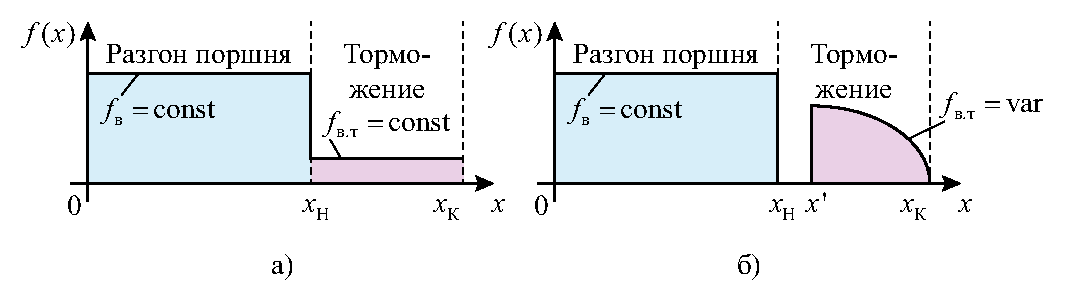
\includegraphics{paroy_brake_mode.eps}
    \caption{Режимы торможения}\label{fig:парой_режимы_торможения}
\end{figure}

Для проектирования тормозных устройств, использующих указанные способы, необходимо определить ряд
параметров, таких как координата начала торможения, площадь сечения выхлопного отверстия,
а также дополнительные координаты и закон изменения площади выхлопа для второго способа.
Автор статьи приводит математические модели, основанные на термодинамических и механических законах,
для расчета этих параметров.

Дальнейшей степенью развития стало комплексное рассмотрение способов торможения ПП в статье <<К вопросу выбора способа торможения
пневмоприводов с большими присоединенными массами>> Г.А. Крутикова, А.И. Кудрявцева и Л.А. Пекаря \cite*{крутиков:способы_торможения_12}
рассмотрено 12 схем торможения ПП, разделенные на 3 основные группы (I, II, III), показанные на рисунке \cref*{fig:эффективные_схемы_торможения_12}.

\begin{figure}[h]
    \centerfloat
    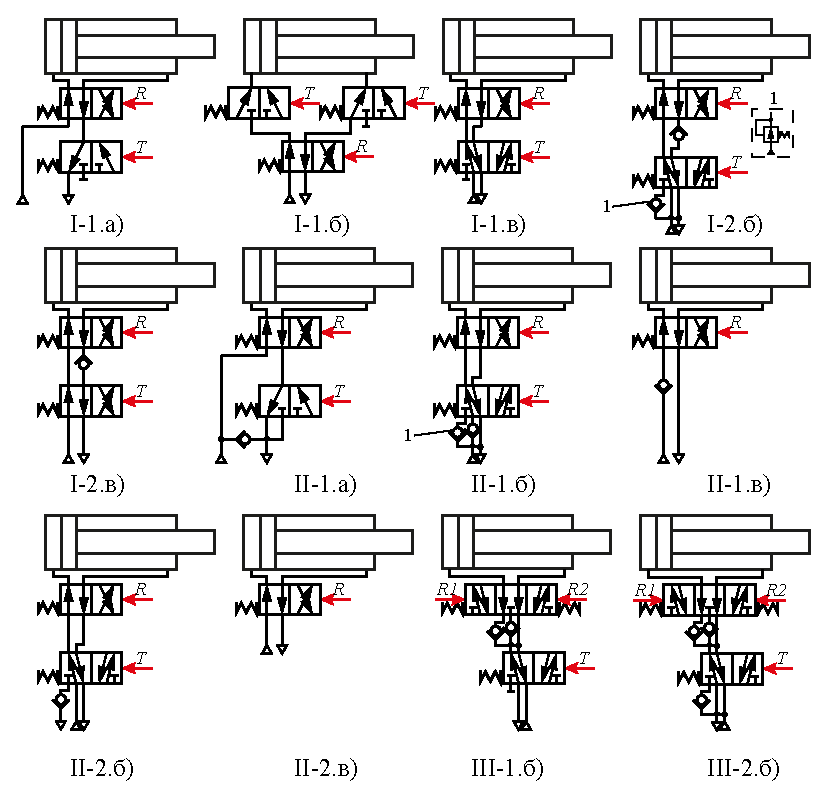
\includegraphics{kurtikob.eps}
    \caption{Эффективные схемы торможения ПП}\label{fig:эффективные_схемы_торможения_12}
\end{figure}

Отличительной особенностью этих схем является отсутствие регулируемых дросселей и емкостей ---
настройка оптимального режима торможения осуществляется только изменением тормозного пути.

Оценка эффективности каждой схемы осуществлялась по ряду ключевых критериев: время срабатывания ПП,
относительная масса сжатого воздуха, потребляемого за один цикл, осредненный за цикл КПД ПП, максимальное
ускорение при торможении, максимальная степень сжатия воздуха в тормозной полости, относительная стоимость
аппаратурной реализации и относительный тормозной путь. Для объективного сравнения каждой схеме была дана оценка в
баллах от 1 до 10 по каждому из показателей, причем максимальный балл присваивался схеме с наилучшим значением
параметра. Коэффициенты весомости различных критериев были определены экспертным методом в соответствии с
рекомендациями.

Наилучшие комплексные показатели качества продемонстрировали схемы III-2.б и III-1.б, которые, несмотря на
более высокую стоимость реализации, обладают лучшими энергетическими характеристиками, высоким быстродействием
и более плавным режимом торможения. Принципиальное отличие этих схем группы III заключается в том, что в них
используется не только вторая составляющая удельной работы сжатого воздуха (изотермическое расширение), но и его
потенциальная энергия, что существенно повышает КПД ПП.

Особого внимания заслуживает схема I-2.б с обратным клапаном, которая позволяет устранить недостатки схемы I-1.б
с высокими пиковыми ускорениями и отскоком поршня. Максимальное ускорение в этом случае снижается с 15,5~\si{\metre\per\square\second}
до 4,16~\si{\metre\per\square\second}, отскок минимален, а время срабатывания составляет 1,05~\si{\second}. Энергетические характеристики также улучшаются
за счет частичной рекуперации воздуха из тормозной полости.

Дальнейшее улучшение режима торможения обеспечивает модификация схемы I-2.б с установкой редукционного клапана вместо
обратного. Это позволяет реализовать практически равнозамедленный режим торможения с постоянным отрицательным
ускорением 1,38~\si{\metre\per\square\second}, полностью устраняет отскок поршня и обеспечивает предохранение тормозной полости от недопустимо
высоких давлений. Основными преимуществами такой схемы являются мягкий и плавный режим торможения с регулируемым
ускорением, экономное использование сжатого воздуха за счет рекуперации, высокое быстродействие и удобство настройки.

Таким образом, комплексная оценка и сравнение различных схем торможения ПП, проведенная авторами, позволила
выявить наиболее эффективные решения. В частности, схема I-2.б с редукционным клапаном демонстрирует оптимальное
сочетание высокого быстродействия, плавного режима торможения с заданным ускорением, экономного расхода сжатого
воздуха и защиты тормозной полости от чрезмерных давлений. Эта схема рекомендуется авторами для использования в качестве
внешнего тормозного устройства для ПП с большими инерционными нагрузками.

Итоговой компиляцией стала работа И.Б. Филипова \cite*{филипов:тормозные_устройства}. В своей монографии, автором подробно рассмотрены конструкции и
принципы построения тормозных устройств, применяемых преимущественно для торможения рабочих органов и звеньев машин
с пневмоприводами. Отмечается, что данные тормозные устройства весьма разнообразны по своему устройству и могут быть
механическими, пневматическими, гидравлическими, электрическими или комбинированными. Механические тормозные устройства
включают в себя пружинные, резиновые, эластомерные, инерционные и фрикционные конструкции, в то время как пневматические
могут быть напорными или вакуумными. Гидравлические тормозные устройства представляют собой устройства дроссельного
регулирования, а к электрическим относятся электромагнитные тормоза с сухим или жидким фрикционным наполнителем.
Кроме того, существуют комбинированные тормозные устройства, сочетающие в себе два или более типов перечисленных.

Автор классифицирует тормозные устройства по виду силовой характеристики или способу
преобразования кинетической энергии подвижных масс, схема классификации представлена на рисунке \cref*{fig:класс_схема_тормозных_устройств}.


\begin{figure}[h]
    \centerfloat
    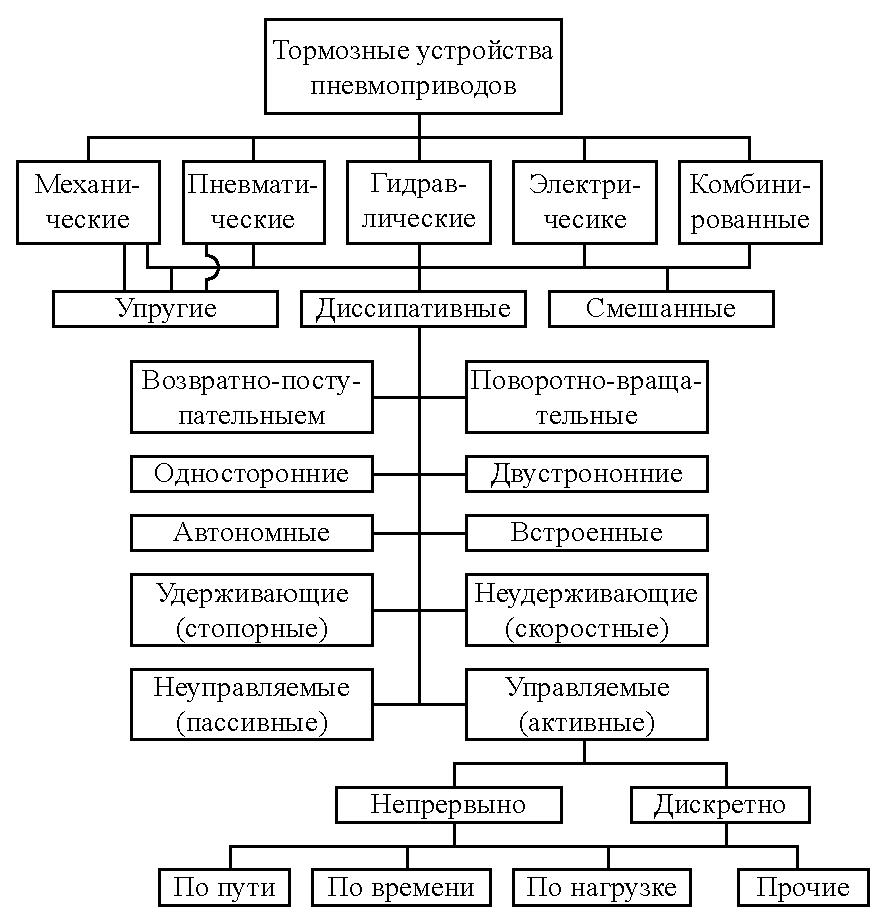
\includegraphics{class_scheme_break.eps}
    \caption{Классификационная схема тормозных устройств}\label{fig:класс_схема_тормозных_устройств}
\end{figure}


Выделяются устройства, создающие упругие,
диссипативные или упруго-диссипативные силы сопротивления. Большинство применяемых в настоящее
время тормозных устройств относятся к последнему типу, частично рассеивающих кинетическую энергию и
частично преобразующих ее в потенциальную. Также тормозные устройства могут быть возвратно-поступательного
или поворотно-вращательного типа движения выходного звена, а по виду действия - одностороннего или двустороннего.

Особое внимание в работе уделено автономным управляемым тормозным устройствам, которые могут быть унифицированы
и использованы для торможения движущихся масс механизмов с различными типами приводов. Их применение существенно
упрощает задачи компоновки и проектирования, а также эксплуатацию и обслуживание промышленного оборудования.
Автор приводит примеры конструктивного исполнения таких тормозных устройств, в том числе встроенных в пневмоцилиндры
для позиционирования выходного звена.

Помимо этого, в работе изложены основные требования к тормозным устройствам, такие как обеспечение заданного закона
торможения, ограничение ускорений, плавность торможения, высокая надежность и быстродействие, простота и компактность
конструкции, стабильность характеристик и другие. Для оценки эффективности применения тормозных устройств предлагается
использовать показатели, основанные на сравнении кинетической энергии, действующих сил, скоростей, ускорений и других
параметров движения выходного звена до и после их внедрения.

Так же, в данной монографии, автор подробно рассматривает особенности позиционных пневматических механизмов
с дискретным управлением, предназначенных для перемещения выходных звеньев или объектов из точки в точку по
заданной программе. Отмечается, что для таких механизмов основными требованиями являются обеспечение максимального
быстродействия и необходимой точности позиционирования при ограниченных динамических нагрузках.

Описывается конструкция и принцип работы разработанного позиционного ПП с одной дискретно управляемой полостью, представленного
на рисунке \cref*{fig:позиционный_пп_филипов}.

\begin{figure}[h]
    \centerfloat
    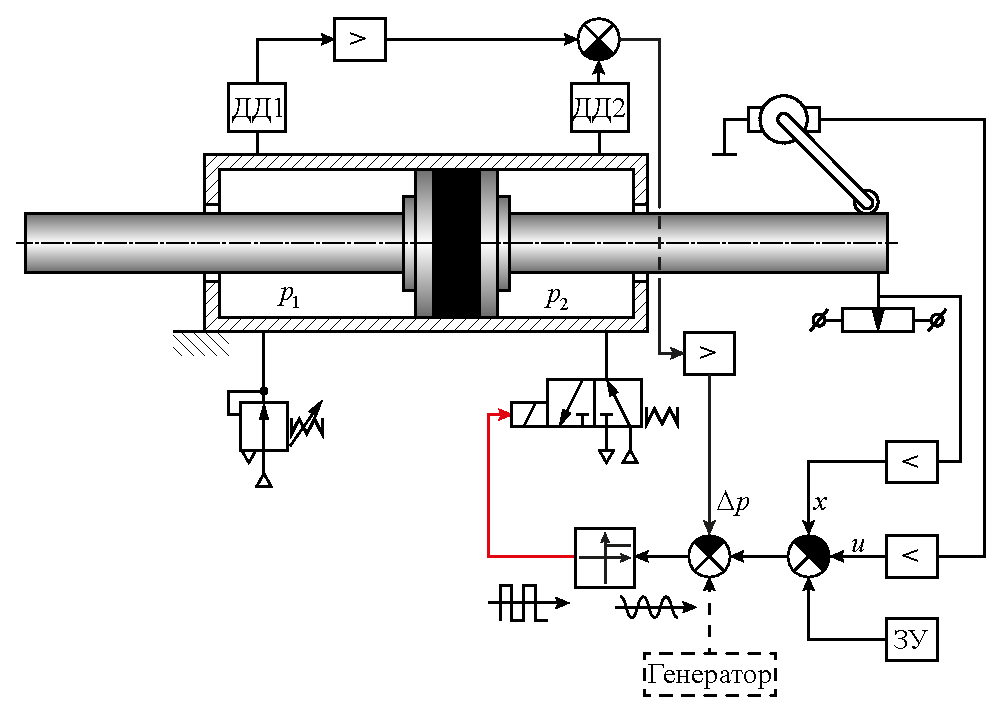
\includegraphics{philipov_positinon_act.eps}
    \caption{Схема дискретного пневмопозиционера}\label{fig:позиционный_пп_филипов}
\end{figure}

Его силовая часть состоит из пневмоцилиндра, в поршневой полости которого через редукционный клапан поддерживается
постоянное давление, а в штоковой полости давление регулируется трехлинейным двухпозиционным клапаном. Измерительная
часть включает датчики давления, тахогенератор и потенциометр для обратных связей по перемещению, скорости и перепаду
давления. Управление движением сводится к управлению торможением и позиционированием за счет переключения клапана,
соединяющего штоковую полость то с магистралью, то с атмосферой.

Автор отмечает, что вследствие колебания давления в штоковой полости уменьшается влияние зоны нечувствительности,
определяемой сухим трением. Приведены результаты исследований, показывающие, что частота переключения клапана определяется
его собственным временем запаздывания и мало зависит от других параметров, что позволяет избежать автоколебаний даже
в наиболее неблагоприятных точках позиционирования.

Дополнительные возможности открывает применение вибрационного сглаживания нелинейностей вынужденными колебаниями.
В этом случае при достижении сигналом рассогласования величины амплитуды гармонического воздействия клапан переходит
в режим постоянного переключения, поддерживая давление в управляемой полости таким, чтобы обеспечить торможение и точное
позиционирование. Преимуществом данного алгоритма является возможность задавать частоту вынужденных колебаний для
обеспечения необходимого качества переходного процесса и требуемого запаса устойчивости.
